%%%%%%%%%%%%%%%%%%%%%%%%%%%%%%%%%%%%%%%%%
% University/School Laboratory Report
% LaTeX Template
% Version 3.1 (25/3/14)
%
% This template has been downloaded from:
% http://www.LaTeXTemplates.com
%
% Original author:
% Linux and Unix Users Group at Virginia Tech Wiki 
% (https://vtluug.org/wiki/Example_LaTeX_chem_lab_report)
%
% License:
% CC BY-NC-SA 3.0 (http://creativecommons.org/licenses/by-nc-sa/3.0/)
%
%%%%%%%%%%%%%%%%%%%%%%%%%%%%%%%%%%%%%%%%%

%----------------------------------------------------------------------------------------
%	PACKAGES AND DOCUMENT CONFIGURATIONS
%----------------------------------------------------------------------------------------

\documentclass{article}

\usepackage[version=3]{mhchem} % Package for chemical equation typesetting
\usepackage{siunitx} % Provides the \SI{}{} and \si{} command for typesetting SI units
\usepackage{graphicx} % Required for the inclusion of images
\graphicspath{ {images/} } % path for images
\usepackage{wrapfig} % places floating figures on the side 
\usepackage{floatrow}
\usepackage{natbib} % Required to change bibliography style to APA
\usepackage{amsmath} % Required for some math elements 

\setlength\parindent{0pt} % Removes all indentation from paragraphs

\renewcommand{\labelenumi}{\alph{enumi}.} % Make numbering in the enumerate environment by letter rather than number (e.g. section 6)

\usepackage{times} % Uncomment to use the Times New Roman font

%----------------------------------------------------------------------------------------
%	DOCUMENT INFORMATION
%----------------------------------------------------------------------------------------

\title{Lab Project: Computer Graphics \\ Building a basic ray tracer \\ SS2017} % Title

\author{Haralambi \textsc{Todorov}} % Author name

\date{\today} % Date for the report

\begin{document}

\maketitle % Insert the title, author and date

\begin{center}
\begin{tabular}{l r}
Advisor: & Prof. Dr.-Ing. Matthias Teschner % Instructor/supervisor
\end{tabular}
\end{center}

% If you wish to include an abstract, uncomment the lines below
% \begin{abstract}
% Abstract text
% \end{abstract}

%----------------------------------------------------------------------------------------
%	SECTION 1
%----------------------------------------------------------------------------------------

\section{Introduction}
\label{sec:intro}

The main objective of the current lab project was to make the author familiar with the basic concepts of a ray tracer by implementing one. This lab report aims to present the gathered knowledge.

\vspace*{\baselineskip}

% explain the structure of the current lab report
The report is split in x chapters with each chapter explaining a certain part of the implemented ray tracer. The ordering of the chapters try to follow the implementation order the author followed during the project. 

\vspace*{\baselineskip}

Current chapter (\ref{sec:intro}) is an introductionary one giving details about the organisation of this report, motivation about why is ray tracing an important rendering technique and where does it find application nowadays along with some information on where do the roots of \textit{ray tracing} come from and the basic idea of the ray tracing algorithm.

\vspace*{\baselineskip}

Chapter (\ref{sec:isects}) deals with one of the fundamental parts of a ray tracer, the ray-object intersection test. It starts with the geometric definition of a half-line (ray), goes on with the diffrent type of geometries the ray tracer supports (spheres, triangles, axis-aligned boxes and triangulated meshes) and how the half-line intersects with these geometries.

\vspace*{\baselineskip}

Chapter (\ref{sec:cameras}) is concerned with how the camera and the image plane are modeled in the ray tracer. It explains the virtual pinhole camera model, how the image plane is mapped within the 3D scene and the two supported camera projections - orthographic and perspective along with their configurable parameters. The chapter goes on with how are rays shot from the image plane and how can one reduce aliasing artefacts by using half-jittered sampling technique. It finishes with the use of gamma correction to enhance the visual apperance of the generated images. 

\vspace*{\baselineskip}



% why should one bother to implement a ray tracer

% some history behind ray tracing

\textit{Ray tracing} is a method of generating an image of an object or scene in which the paths of light rays (usually in reverse, from the camera or the eye to the object) are estimated by computer. \cite{oxford_dict} 

% show image from movie
\begin{figure}[h!]
    \caption{A shot from the movie "Finding Dory" ray traced with Pixar's Renderman. 2016 Pixar. All Rights Reserved.}
    \centering
    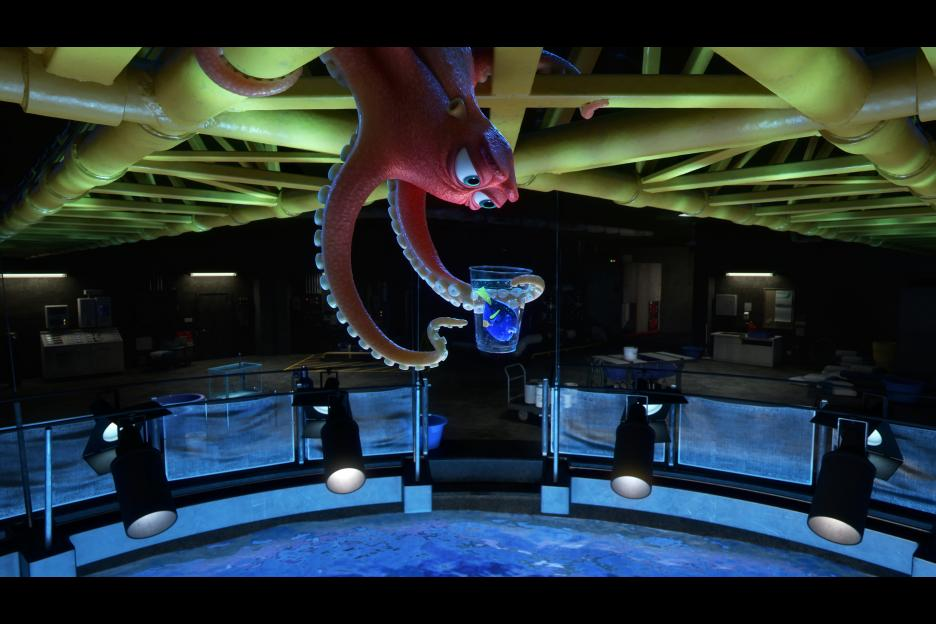
\includegraphics[width=0.8\textwidth]{finding_dory_shot}
    \label{fig:finding_dory}
\end{figure}

This rendering technique is prefered from multiple industries such as entertainment or science for its capabilities to create photorealistic images easily incorporating complex physical effects like caustics, reflections and refractions. One could see an example of a ray taced image with reflections and refractions on figure \ref{fig:finding_dory} made with Pixar's \textit{RenderMan}.

\vspace*{\baselineskip}

The first ray tracing algorithm was introduced by Arthur Appel in 1968, which idea was to shoot from the eye, one per pixel, and find the closest object blocking the path of that ray. Using the material properties and the effect of the lights in the scene, this algorithm can determine the shading of objects. \cite{appel} 

%----------------------------------------------------------------------------------------
%	SECTION 2
%----------------------------------------------------------------------------------------

\section{Experimental Data}


%----------------------------------------------------------------------------------------
%	SECTION 3
%----------------------------------------------------------------------------------------

\section{Sample Calculation}

%----------------------------------------------------------------------------------------
%	SECTION 4
%----------------------------------------------------------------------------------------

\section{Results and Conclusions}

%----------------------------------------------------------------------------------------
%	SECTION 5
%----------------------------------------------------------------------------------------

\section{Discussion of Experimental Uncertainty}

%----------------------------------------------------------------------------------------
%	SECTION 6
%----------------------------------------------------------------------------------------

\section{Answers to Definitions}

%----------------------------------------------------------------------------------------
%	BIBLIOGRAPHY
%----------------------------------------------------------------------------------------

\bibliographystyle{alpha}
\bibliography{sample}

%----------------------------------------------------------------------------------------

\end{document}